\documentclass[french]{article}
\usepackage[T1]{fontenc}
\usepackage{fullpage}
\usepackage{babel}
\usepackage{hyperref}
\usepackage{graphicx}
\usepackage[justification=centering]{caption}
\usepackage{amsmath}
\usepackage{amssymb}
\usepackage{spverbatim}

\hypersetup{
  colorlinks=true,
  linkcolor=black,
  urlcolor=blue
}

\graphicspath{ {./img/} }
\title{%
    \huge Your News Anchor  \\
    \bigskip
    \large E1 - Mise en situation \\ 
    Développeur en Intelligence Artificielle,
    titre professionnel enregistré au RNCP - École IA Microsoft by Simplon
    \vfill
    
\includegraphics[width=14cm]{cover.jpg} 
    \vfill}
\date{9 février 2024}
\author{par Vincent Papelard}

\begin{document}
    \renewcommand{\contentsname}{Table des Matières}
    \maketitle
    \pagenumbering{arabic}
    \pagenumbering{gobble}
    \newpage
    \tableofcontents
    \newpage
    \pagenumbering{arabic}

    \section*{Introduction}
    Dans un contexte de diffusion rapide de l'information via Internet et face à la multitude de sources d'informations disponibles, il est parfois difficile de savoir où s'informer. Où trouver les actualités qui nous intéressent vraiment, en allant à l'essentiel ? C'est la problématique à laquelle répond ce projet qui nous est confié par notre client, un gros acteur dans le domaine des médias.
    
    \textbf{Your News Anchor} est une application web qui offre à ses utilisateurs un résumé concis des actualités du jour. Ce résumé est automatiquement généré par intelligence artificielle à l'aide d'une liste de sources personnalisable par l'utilisateur, puis présenté par une voix synthétisée comme un vrai journal télévisé.
    Ce dossier se penche sur toute la partie du projet relative à la collecte, au nettoyage et au stockage des données nécessaires à la génération automatique de résumés. \textbf{Le développement de l'application à proprement parler ainsi que la conception d'un modèle d'intelligence artificielle de génération de résumé ne sont pas couverts dans ce dossier}.
    La totalité du code est disponible sur GitHub :
    \begin{itemize}
        \item Collecte, nettoyage et aggrégation des données : \url{https://github.com/vinpap/your_news_anchor}
        \item API de la base de données : \url{https://github.com/vinpap/your_news_anchor_db_api}
    \end{itemize}

    Notre client souhaite que le projet soit terminé dans un délai d'un mois. Pour cela, il nous alloue un budget de 4200€. Ce budget couvre uniquement nos honoraires, soit 21 jours travaillés facturés 200€ chacun. Tous les frais réguliers qui devront être payés suite à la livraison du projet, tels que le paiement d'abonnement à des services de cloud, sont à la charge de notre client. 
    \addcontentsline{toc}{section}{Introduction}

    \section{Présentation des outils, plateformes et langages utilisés}

    Les outils et plateformes suivants ont été utilisés dans le cadre de ce projet :
    \begin{itemize}
        \item Développement : \textbf{Python}
        \item Base de données : \textbf{PostgreSQL}
        \item Visualisation de la base de données : \textbf{\href{https://dbeaver.io/}{DBeaver}}
        \item Plateformes de déploiement : \textbf{\href{https://azure.microsoft.com/fr-fr}{Microsoft Azure}}, \textbf{\href{https://www.pythonanywhere.com/}{PythonAnywhere}}
        \item Versionnage et gestion de projet : \textbf{GitHub}
        \item Prise de notes : \textbf{\href{https://obsidian.md/}{Obsidian}}
        \item Rédaction du rendu : \textbf{\LaTeX} 
        \item Diagrammes et schémas : \textbf{\href{https://app.diagrams.net/}{draw.io}}
    \end{itemize}
    
    \section{Gestion du projet}
    Le projet a été réalisé au cours de plusieurs sprints d'une semaine chacun. GitHub a été utilisé pour assurer le suivi des tâches et des sprints, ainsi que le versionnage du code.
    
    \begin{figure}[h]
        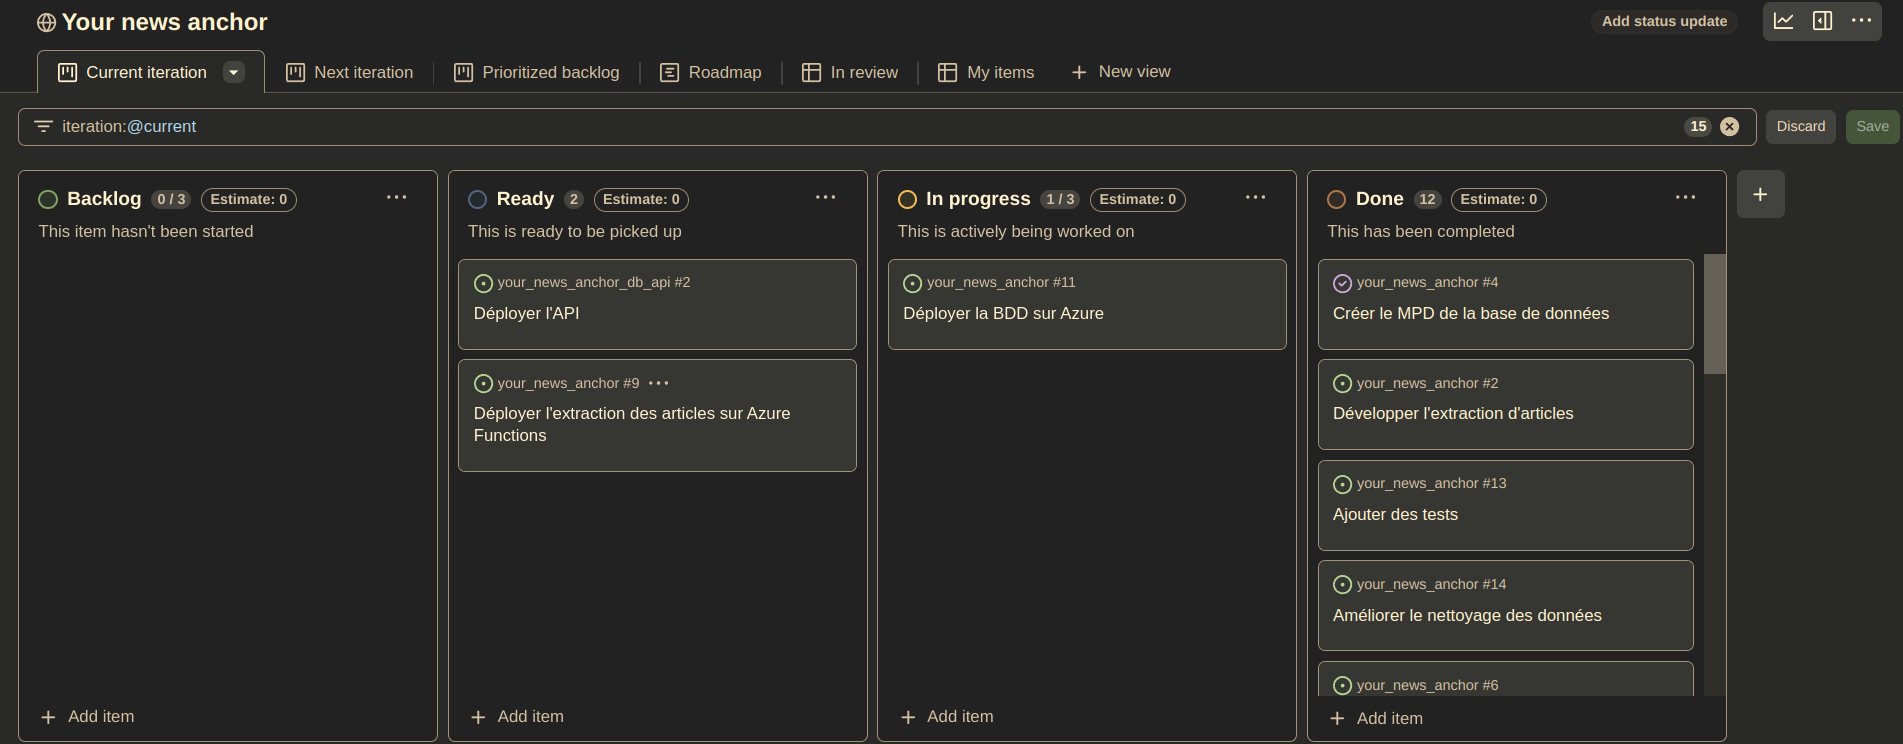
\includegraphics[width=12cm]{gh_projects}
        \centering
        \caption{Tableau des tâches de GitHub Projects}
        \centering
    \end{figure}

    \section{Les composants du projet}
    Le projet est divisé en trois composants : 
    \begin{itemize}
        \item une \textbf{base de données} PostgreSQL hébergée sur Azure qui stocke les sources d'information et les articles de journal extraits ainsi que les informations concernant les utilisateurs de \textit{Your News Anchor}
        \item une \href{https://github.com/vinpap/your_news_anchor_db_api}{API} qui expose cette base de données
        \item le script \href{https://github.com/vinpap/your_news_anchor/blob/main/extract_articles.py}{extract\_articles.py}. Ce script effectue \textbf{la collecte, le nettoyage et l'aggrégation des articles de journal qui nous serviront à générer des résumés}, avant de les stocker dans la base de données en passant par l'API.
    \end{itemize}
    Chaque composant est développé et déployé indépendamment des deux autres, selon une architecture de microservices. Les différentes étapes de l'exécution du projet sont détaillées dans la figure 2. Par ailleurs, des \textbf{\hyperref[img:screenshots_processus]{captures d'écran}} sont présentées dans les annexes pour illustrer les diférentes étapes du processus.
    \begin{figure}[h]
        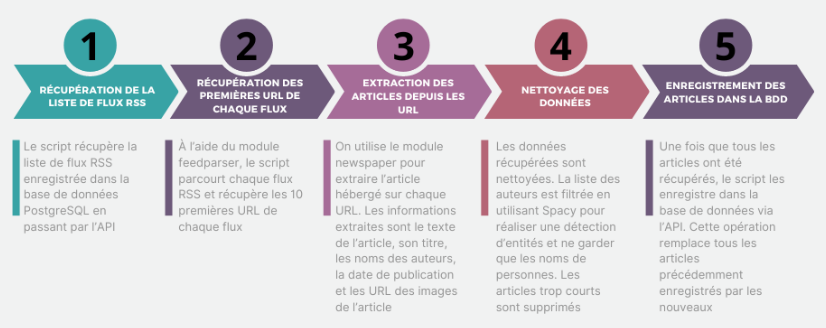
\includegraphics[width=15cm]{fonctionnement_script}
        \centering
        \caption{Fonctionnement général du projet, de la récupération de la liste des sources d'information à utiliser à l'enregistrement des articles extraits dans la base de données.}
        \centering
    \end{figure}
    
    \subsection{Collecte des données}

    La collecte des données est réalisée par le script \href{https://github.com/vinpap/your_news_anchor/blob/main/extract_articles.py}{extract\_articles.py}, qui fait lui-même appel à des fonctions définies dans \href{https://github.com/vinpap/your_news_anchor/blob/5deffe3be7453d998b2377548902759869e1926d/extraction_functions.py}{extraction\_functions.py}. Afin que les articles stockés dans la base de données restent à jour, ce script est \textbf{automatiquement exécuté toutes les 24 heures} pour récupérer les derniers articles de journaux publiés.
    
    La collecte des données est réalisée en plusieurs étapes. Tout d'abord, le script appelle l'API pour récupérer une liste de sources d'information d'où extraire des articles \href{https://github.com/vinpap/your_news_anchor/blob/5deffe3be7453d998b2377548902759869e1926d/extract_articles.py#L37}{\textbf{(lien vers le code)}}.

    On va ensuite utiliser le module \textbf{\href{https://pypi.org/project/feedparser/}{feedparser}} de Python pour parcourir les flux RSS et en extraire une liste d'URLs d'articles avec d'autres informations telles que le titre de chaque article. Dans la mesure où l'objectif final est de réaliser des résumés concis des actualités du jour, on ne récupère pas la totalité des articles de chaque flux RSS. À la place on récupère les n premiers articles de chaque flux (les premiers articles correspondent souvent aux gros titres du jour, et ont donc plus de chance d'être pertinents).
    Enfin, on récupère le code HTML des pages web de chaque article et on en extrait le texte de l'article ainsi que plusieurs métadonnées utiles (auteurs, date de publication...). 

    Cette étape représente un défi particulier. En effet, l'approche traditionnelle consiste à identifier dans le code HTML les classes et id qui permettent de localiser sur la page web le contenu que l'on souhaite extraire, en utilisant des outils tels que BeautifulSoup. Or, la structure de chaque page web est différente. Si l'on voulait collecter le contenu des articles de façon fiable, il faudrait techniquement écrire du code propre à chaque site web. Cette approche a plusieurs inconvénients qui la rendent inadaptée à nos besoins :
    \begin{itemize}
        \item Écrire un code différent pour chaque source de données est un travail long et laborieux. De plus certains sites nous compliquent la tâche, par exemple en obfusquant les noms des classes et des id dans leur code source
        \item L'application prévoit que les utilisateurs puissent eux-mêmes rajouter des sources de données. Cela est impossible si le code ne nous permet de gérer qu'une liste de sites web fixe
        \item Par ailleurs, cette technique est très peu robuste. Le moindre changement apporté au code source des pages web peut rendre notre code obsolète.
    \end{itemize}
    Pour toutes ces raisons, on préfèrera s'orienter vers d'autres méthodes. L'idéal serait de pouvoir coder un "web scraper universel", qui nous permettrait d'extraire le texte de n'importe quel article publié sur une page web quelconque. Cette tâche est extrêmement difficile à mettre en place en pratique, mais il est néanmoins possible de s'en approcher grâce au package Python \textbf{\href{https://newspaper.readthedocs.io/en/latest/}{newspaper}}, qui est utilisé dans le cadre de ce projet.
    Newspaper est un package créé pour extraire et traiter des articles depuis des pages web. Il permet ainsi d'extraire un article depuis une page web en quelques lignes :
    \begin{verbatim}
        from newspaper import Article

        url = 'https://url-de-votre-article.com'
        article = Article(url)
        article.download()
        article.parse()
        text = article.text
    \end{verbatim}
    Newspaper fonctionne en analysant le code des pages web avec BeautifulSoup. Certaines informations (titre, date...) sont retrouvées en cherchant des balises spécifiques telles que la balise <h1> par exemple, où grâce à des expressions régulières. Newspaper extrait aussi d'autres informations telles que les mots-clés d'un article grâce au module de NLP nltk. Dans notre cas, on récupérera les informations suivantes :
    \begin{itemize}
        \item le texte de l'article
        \item les auteurs
        \item la date de publication
        \item l'url de l'image en une de l'article (s'il y en a une)
    \end{itemize}
    Il est important de noter que cette solution n'est pas parfaite. Certains types de contenu, tels que les vidéos, ne sont pas exploitables. Newspaper a aussi du mal à traiter certains sites particuliers (il échoue à récupérer les articles du site 'L'Équipe', par exemple). Malgré tout, les résultats obtenus ont été concluants avec la grande majorité des sites d'information testés, en français comme en anglais.

    \subsection{Nettoyage des données}
    Le nettoyage des données est également réalisé par le script \href{https://github.com/vinpap/your_news_anchor/blob/main/extract_articles.py}{extract\_articles.py}.
    Après avoir collecté les articles, le script Python va passer par une étape de nettoyage des données. Malgré la bonne qualité générale du texte extrait, certains types de texte ne sont pas exploitables pour générer des résumés :
    \begin{itemize}
        \item Les reportages vidéo, qui ne comportent généralement qu'un bref texte de description sous la vidéo
        \item Les articles réservés aux abonnés, où seul le début du texte est visible
        \item Les flashs info et autres articles très (trop) courts pour en faire un résumé, de manière générale.
    \end{itemize}
    Les noms des auteurs automatiquement extraits par newspaper posent également problème. La liste d'auteurs générée identifie souvent de façon erronnée des auteurs dans le corps de l'article, et il n'est pas rare d'obtenir des listes d'auteurs telles que ['Par', 'Julien Dupont', 'Le Président'], par exemple.

    Le premier problème peut être résolu simplement : il suffit de filtrer les articles en fonction de leur longueur, pour ne garder que ceux dont le nombre de caractères dépasse une certain seuil.
    En ce qui concerne la liste des auteurs, une solution un peu plus complexe a été trouvée : réaliser une détection d'entités dans la liste à l'aide de \textbf{\href{https://spacy.io/}{Spacy}} pour ne garder que les chaînes de caractère qui correspondent à des noms propres qui désignent des persones. Cela a permis d'éliminer la quasi-totalité des erreurs d'extraction de noms d'auteur.

    Après avoir été nettoyés, les articles extraits sont \href{https://github.com/vinpap/your_news_anchor/blob/5deffe3be7453d998b2377548902759869e1926d/extract_articles.py#L51}{rassemblés dans une liste Python} avant d'être enregistrés via une API dans la base de données décrite dans la section suivante.

    \subsection{Stockage des données}

    Toutes les informations extraites (articles et métadonnées) ainsi que la liste des sources d'information à traiter et toutes les autres données nécessaires au fonctionnement de l'application Your News Anchor sont stockées sur une base de données \textbf{PostgreSQL}. Le Modèle Physique de Données qui décrit la structure de notre base de données est présenté dans la figure 3.

    \begin{figure}[h]
        \includegraphics[width=12cm]{mpd_e1}
        \centering
        \caption{MPD de notre base de données}
        \centering
    \end{figure}


    La base de données est composée des tables suivantes :
    \begin{itemize}
        \item \textit{standard\_sources} : contient une liste de sources d'information, avec le lien vers leur flux RSS. Cette liste est définie par les administrateurs de l'application et ne peut pas être modifiée par les utilisateurs. Les flux RSS disponibles dans cette table peuvent être utilisés par n'importe quel utilisateur
        \item \textit{user\_sources} : cette table recense les flux RSS ajoutés manuellement par les utilisateurs. Seul l'utilisateur qui a ajouté un flux peut l'incorporer dans sa liste de sources d'informations
        \item \textit{users} : la table qui contient les informations concernant les utilisateurs (identifiant, hash du mot de passe...)
        \item \textit{daily\_articles} : contient tous les articles extraits par le script de collecte des données. Le contenu de cette table est renouvelé à intervalles réguliers (par exemple toutes les 24 heures), lorsque le script de collecte des données est exécuté
        \item \textit{daily\_recaps} : la table où sont stockés les résumés d'articles générés. Ces résumés sont eux aussi renouvelés à intervalles réguliers.
    \end{itemize}

    Différentes requêtes et insertions SQL sont utilisées pour réaliser les tâches suivantes :
    \begin{itemize}
        \item Récupération de la liste des flux RSS disponibles pour un utilisateur spécifique
        \item Récupération de la liste de tous les flux RSS enregistrés
        \item Mise à jour des articles de journal enregistrés dans la base de données avec une nouvelle liste d'articles.
    \end{itemize} 
    Une liste complète des requêtes SQL utilisées dans le cadre de ce projet est disponible \textbf{\hyperref[sec:sql]{en annexe}}.
    On notera que ces requêtes ont été pensées pour optimiser la vitesse d'accès aux données. Ainsi :
    \begin{itemize}
        \item L'ancien contenu de la table \textit{daily\_articles} est supprimé avant d'y insérer les articles de journal du jour. L'objectif est de ne garder que des articles pertinents et de limiter la taille de cette table, ce qui accélère l'exécution des requêtes sur cette table
        \item On modifie les requêtes pour ne sélectionner dans les tables que les informations dont on a besoin. Dans la \textbf{\hyperref[sec:query]{requête qui sélectionne la liste des flux RSS disponibles pour un utilisateur}}, par exemple, on nomme explicitement toutes les colonnes que l'on veut sélectionner dans notre requête plutôt que de tout sélectionner en utilisant 'SELECT *', qui est plus lent. À titre d'exemple, le temps d'exécution de la requête ci-dessus est passé de 18 ms à 15 ms en effectuant ce changement, avec environ dix lignes dans la table \textit{user\_sources} et la table \textit{standard\_sources}.
    \end{itemize} 
    

    On notera que ces requêtes ne sont en aucun cas utilisées par notre script extract\_articles.py, qui n'a pas accès à la base de données. À la place, le script accède à la base de données en passant par une API que nous allons présenter dans la section suivante. Cette API est définie dans un dépôt séparé, dans un script \textbf{app.py} (\href{https://github.com/vinpap/your_news_anchor_db_api/blob/main/app.py}{lien}). C'est ce script qui exécute les insertions et requêtes SQL présentées dans les annexes.
    
    \subsection{Accès aux données et API}
    
    Afin de simplifier l'accès aux données, une API a été développée pour exposer la base de données PostgreSQL. Cela nous évite de devoir gérer nous-mêmes les connexions et requêtes SQL dans notre application, et nous permet de mettre en place des sécurités pour contrôler qui accède à nos données et/ou les modifie.
    L'API a été développée à l'aide de \textbf{\href{https://fastapi.tiangolo.com/}{FastAPI}}, un framework Python destiné à développer rapidement des API REST performantes. Cette API propose deux endpoints pertinents dans le cadre de notre dossier :
    \begin{itemize}
        \item \textbf{/feeds}, qui permet de récupérer (mais pas de modifier) le contenu de la table 'sources'
        \item \textbf{/update\_articles}, qui sert à renouveler entièrement le contenu de la table 'daily\_articles'. Cette opération implique d'effacer le contenu existant de la table pour le remplacer par les données envoyées dans un objet JSON joint à la requête.
    \end{itemize}

    Dans la mesure où la requête envoyée à ce deuxième endpoint supprime des données, il a fallu sécuriser l'accès à la base de données. Dans ce but, une clé d'API secrète doit étre envoyée avec la requête. Cette clé est stockée dans une variable d'environnement afin de ne pas être visible "en clair" sur un dépôt GitHub, par exemple. Plus d'informations sont disponibles dans la section consacrée au déploiement du projet.

    \section{Tests et intégration continue}
    Afin de garantir la qualité du code et de s'assurer que ni notre script extract\_articles.py ni le script de notre API app.py ne vont cesser de fonctionner, plusieurs mesures ont été prises :
    \begin{itemize}
        \item des tests unitaires ont été codés dans le fichier \href{https://github.com/vinpap/your_news_anchor/blob/main/test/test_extraction_script.py}{test\_extraction\_script.py} pour vérifier que les fonctions qui permettent d'extraire les articles de journaux de pages web fonctionnent bien comme attendu. De la même manière, le \href{https://github.com/vinpap/your_news_anchor_db_api/blob/main/test_api.py}{fichier test\_api.py} contient des tests unitaires qui vérifient que les différents points de terminaison de l'API fonctionnent comme attendu.
        \item ces tests ont été automatisés avec GitHub Action. Ils sont ainsi automatiquement exécutés à chaque fois que du code est intégré à la branche 'main' du dépôt 'your\_news\_anchor' ou du dépôt 'your\_news\_anchor\_db\_api'.
    \end{itemize}
    \section{Déploiement}
    Comme évoqué plus haut, les trois composants de ce projet sont développés et déployés indépendamment les uns des autres.
    \subsection{Base de données}
    La base de données PostgreSQL a d'abord été mise en place localement pendant la période de développement. Elle a ensuite été exportée via un script SQL accessible via \href{https://github.com/vinpap/your_news_anchor_db_api/blob/main/create_db.sql}{ce lien} sur le service Azure Database for PostgreSQL de Microsoft Azure. 
    Pour plus de sécurité, la base de données a été paramétrée de sorte à n'autoriser l'accès qu'à une adresse IP spécifique, où est déployée notre API.

    \subsection{API}

    L'API est elle aussi déployée sur Microsoft Azure, plus spécifiquement sur le service \textbf{Azure Web App}. Le déploiement est automatisé grâce à GitHub Actions afin que les mises à jour apportées au code soient automatiquement déployées sur Azure.
    Comme nous l'avons vu, l'API a besoin de définir une clé secrète pour fonctionner. Cependant, il est impossible d'inclure cette clé dans notre code pour des raisons évidentes : celle-ci serait visible de tous sur notre dépôt GitHub. Pour régler ce problème, on utilisera des secrets GitHub. Cette fonctionnalité de GitHub nous permet de créer des valeurs secrètes lieés à notre dépôt mais dont la valeur est cachée. On peut ensuite ajouter les lignes suivantes au fichier YAML qui gère le pipeline de déploiement de GitHub action : 
    \begin{verbatim}
        - name: Create secret values in environment (APi token and DB password)
        run: |
          export API_TOKEN=${{ secrets.SECRET_API_TOKEN }}
          export DB_PWD=${{ secrets.SECRET_DB_PWD }}
    \end{verbatim}

    Lors du déploiement, ces instructions créeront sur le serveur des variables d'environnement qui contiennent nos valeurs secrètes (le mot de passe de la base de données et notre token d'API) sans pour autant exposer leur valeur dans le code.

    \subsection{Script d'extraction des données}

    Notre script d'extraction d'articles doit être automatiquement exécuté à intervalles réguliers. La solution retenue a été de l'exécuter sur \textbf{\href{https://www.pythonanywhere.com/}{PythonAnywhere}}. PythonAnywhere est une plateforme basée sur AWS qui permet de déployer des scripts et applications Python avec un minimum d'efforts.

    \section*{Conclusion}

    Ce dossier a couvert toutes les problématiques liées à la mise à disposition des données dans le cadre du projet Your News Anchor. Il a notamment mis en évidence les difficultés liées à la mise en place d'une solution de web scraping universel, et les réponses qui peuvent être apportées à ce problème. L'utilisation de packages tels que newspaper, qui combinent techniques de NLP et analyse de code HTML, en est un exemple.
    \addcontentsline{toc}{section}{Conclusion}


    \appendix
    \newpage
    \section*{Annexes \huge \centering}
    \addcontentsline{toc}{section}{Annexes}
    \section*{Illustration de l'exécution du projet}
    \label{img:screenshots_processus}
    \begin{figure}[h!]
        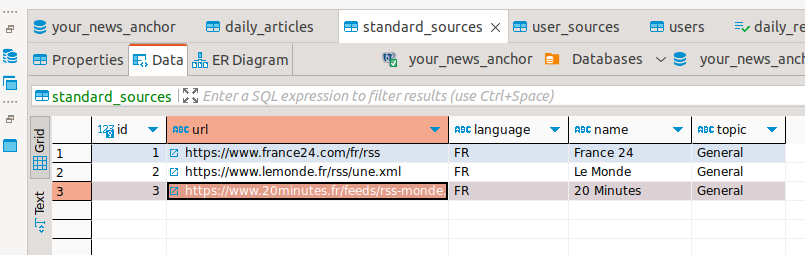
\includegraphics[width=12cm]{db_1}
        \centering
        \caption{Notre base de données PostgreSQL stocke une liste de flux RSS à utiliser pour récupérer les adresses web d'articles de journaux. Cette capture d'écran montre la table 'standard\_sources' qui contient une liste de flux RSS disponibles pour tous les utilisateurs, mais ces derniers peuvent aussi ajouter leur propre liste de flux RSS qui seront stockés dans la table 'user\_sources'.}
        \centering
    \end{figure}
    \begin{figure}[h!]
        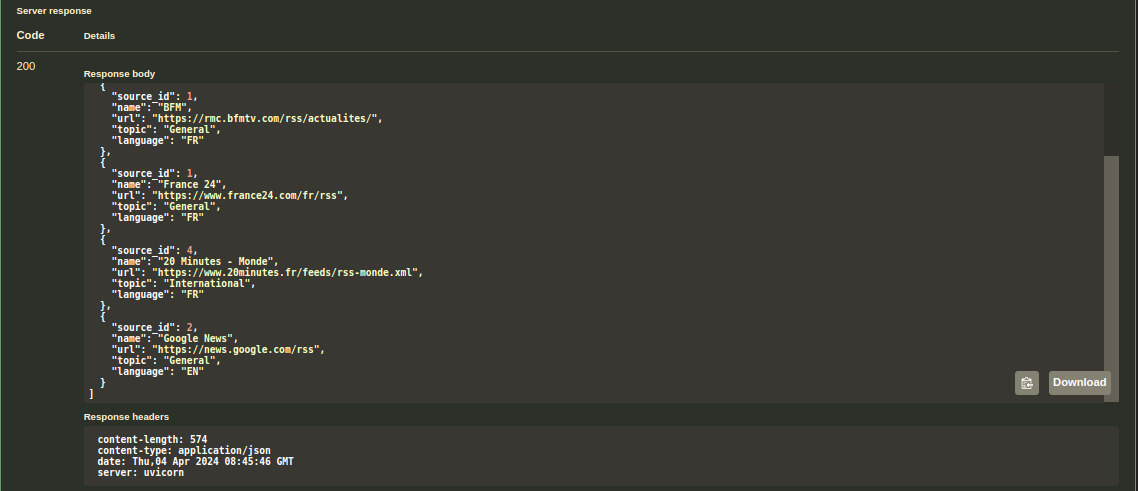
\includegraphics[width=12cm]{api_1}
        \centering
        \caption{Le script extract\_articles.py accède à la base de données via une API. Cette image montre le résultat d'une requête envoyée à l'API pour récupérer la liste des sources d'information à utiliser pour un utilisateur spécifique. Ces sources sont soit des sources 'standard', c'est-à-dire que tous les utilisateurs y ont accès, soit des sources personnalisées que l'utilisateur a lui-même enregistrées.}
        \centering
    \end{figure}
    \begin{figure}[h!]
        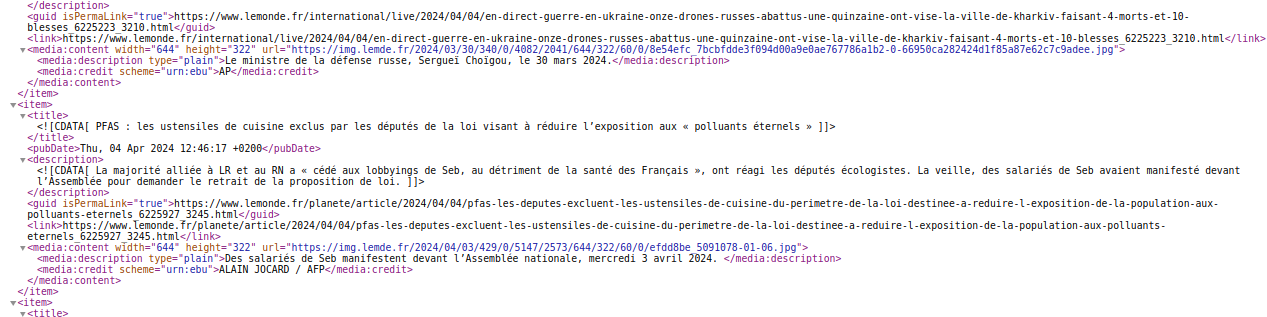
\includegraphics[width=12cm]{rss}
        \centering
        \caption{Les flux RSS nous permettent de récupérer les adresses web des derniers articles publiés sur un site d'information. Cette capture d'écran nous montre une partie du flux RSS du site du journal Le Monde.}
        \centering
    \end{figure}
    \begin{figure}[h!]
        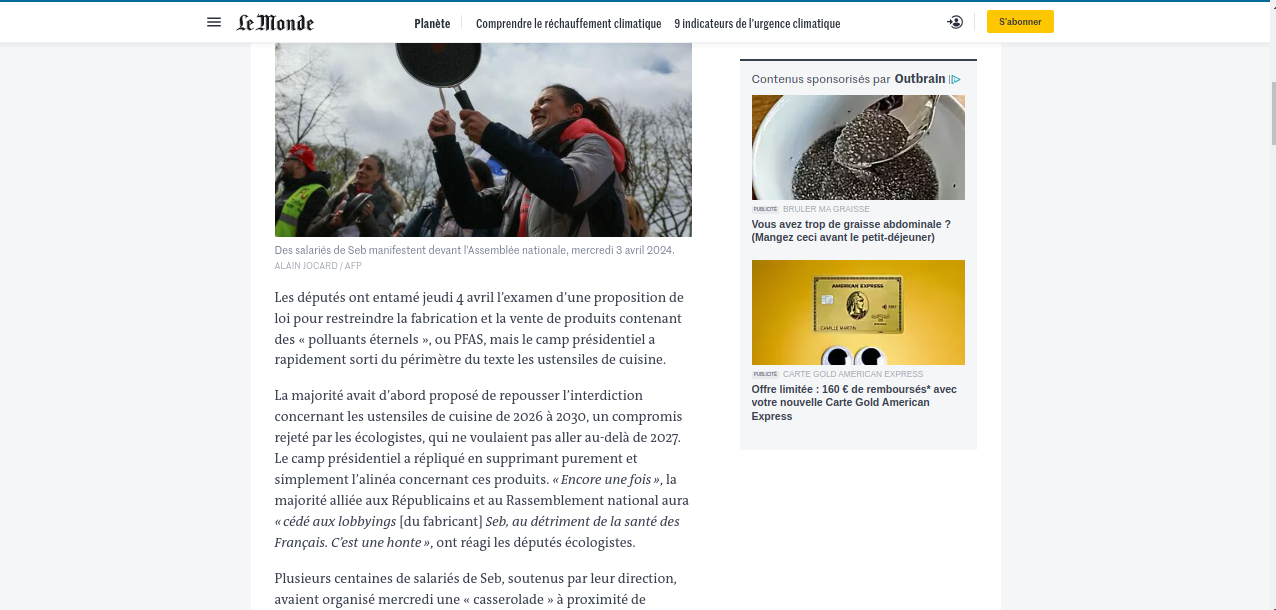
\includegraphics[width=12cm]{original_website}
        \centering
        \caption{Le flux RSS présenté ci-dessus permet à notre script extract\_articles.py d'accéder à l'article suivant.}
        \centering
    \end{figure}
    \begin{figure}[h!]
        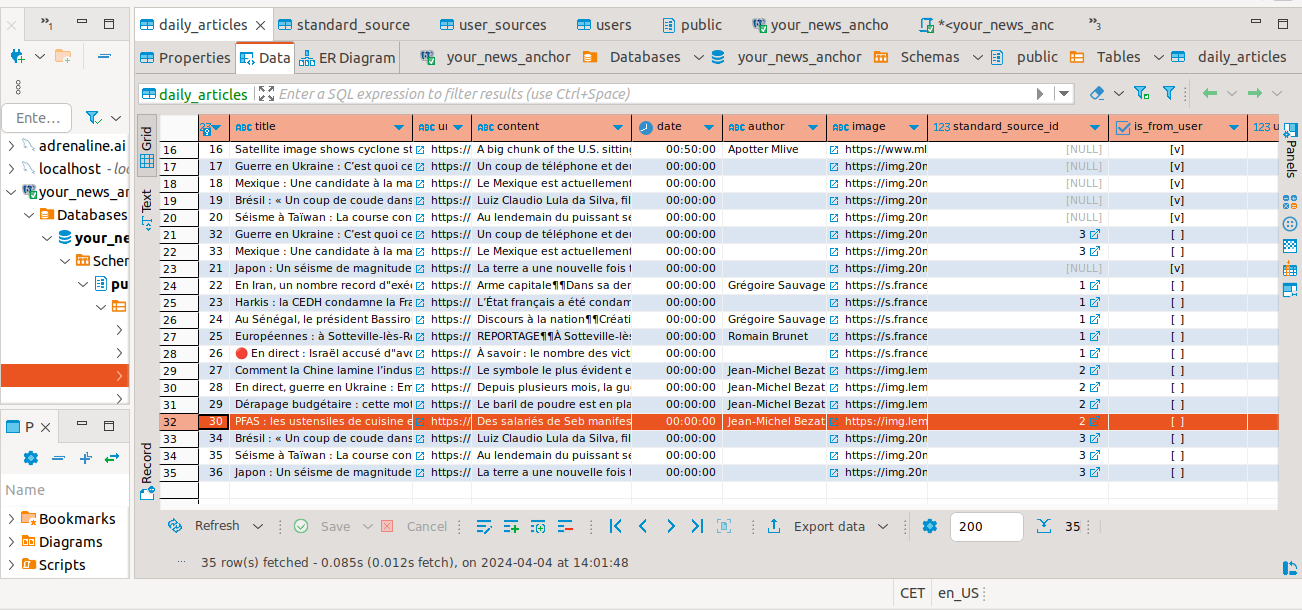
\includegraphics[width=12cm]{db_2}
        \centering
        \caption{Après avoir extrait et nettoyé le contenu de l'article depuis la page web, le script extract\_articles.py enregistre les articles extraits dans la base de données via le point de terminaison '/update\_articles' de l'API. Cette capture d'écran montre le contenu de la table 'daily\_articles' dans la base de données, incluant l'article de journal ci-dessus.}
        \centering
    \end{figure}
    \section*{Architecture générale du projet}
    \begin{figure}[h!]
        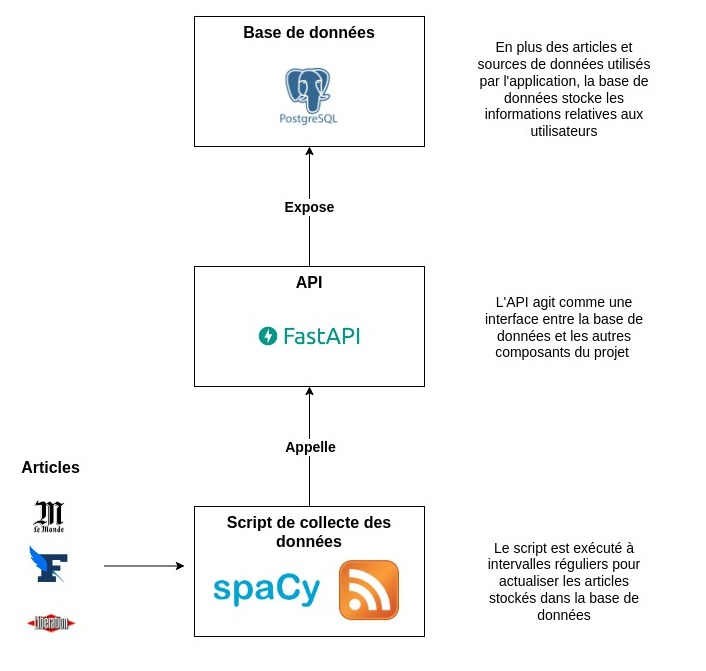
\includegraphics[width=12cm]{composants}
        \centering
        \caption{Les différents composants du projet}
        \centering
    \end{figure}
    \section*{Sources de données utilisées pour les tests}
    Voici la liste des flux RSS avec lesquels l'extraction de données a été testée avec succès pendant le développement :
    \begin{itemize}
        \item https://www.france24.com/fr/rss
        \item https://www.lemonde.fr/rss/une.xml
        \item https://news.google.com/rss?hl=fr\&gl=FR\&ceid=FR:fr
        \item https://www.ouest-france.fr/rss/france
        \item https://www.francetvinfo.fr/monde.rss
        \item https://www.20minutes.fr/feeds/rss-monde.xml
        \item https://rmc.bfmtv.com/rss/actualites/
        \item https://feeds.leparisien.fr/leparisien/rss
        \item https://www.ladepeche.fr/rss.xml
    \end{itemize}
    En plus des sources ci-dessus, le script a été testé avec le flux RSS du journal l'Équipe. Les résultats n'ont pas été concluants (Seul les premières phrases de chaque article sont détectées).
    
    Plusieurs flux RSS de sources en anglais ont aussi été testés, avec succès :
    \begin{itemize}
        \item https://www.independent.co.uk/news/world/rss
        \item https://rss.app/feeds/D0SUH2NYYoOzypYN.xml
        \item https://www.huffpost.com/section/world-news/feed
        \item https://news.google.com/rss
    \end{itemize}
    \section*{SQL}
    \label{sec:sql}
    Voici la liste des requêtes et insertions SQL utilisées par l'API \href{}{'your\_news\_anchor\_db\_api} dans le cadre de ce projet :
    \begin{itemize}
        \label{sec:query}
        \item point de terminaison /feeds : récupération de la liste des flux RSS disponibles pour un utilisateur
        \begin{itemize}
            \item Pour vérifier que l'utilisateur concerné existe bien :
            \begin{verbatim}
            SELECT * FROM users WHERE username='{username}';
            \end{verbatim}
            \item Pour récupérer l'identifiant de l'utilisateur :
            \begin{verbatim}
            SELECT id from users where username='{username}';
            \end{verbatim}
            \item Pour récupérer la liste des flux RSS disponibles :
            \begin{spverbatim}
            SELECT url, language, topic, name FROM (select url, language, topic, name from user_sources where user_id={user_id}) union  (select url, language, topic, name from standard_sources where not exists (select * from user_sources where user_sources.url=standard_sources.url));
            \end{spverbatim}
        \end{itemize}
        \item point de terminaison /all\_feeds : récupération de la liste de tous les flux RSS enregistrés
        \begin{itemize}
            \item Récupération des flux RSS enregistrés par les utilisateurs :
            \begin{spverbatim}
            SELECT id, url, language, topic, name FROM user_sources;
            \end{spverbatim}
            \item Récupération des flux RSS disponibles pour tous les utilisateurs :
            \begin{spverbatim}
            SELECT id, url, language, topic, name from standard_sources;
            \end{spverbatim}
        \end{itemize}
        \item point de terminaison /update\_articles : mise à jour des articles stockés dans la base de données
        \begin{itemize}
            \item Sélection des identifiants de tous les articles déjà enregistrés, permet d'identifier les articles obsolètes qui doivent être supprimés après l'ajout des nouveau articles :
            \begin{spverbatim}
            SELECT id FROM daily_articles;
            \end{spverbatim}
            \item Insertion des nouveaux articles :
            \begin{spverbatim}
            INSERT INTO daily_articles(title, url, content, author, image, is_from_user, user_source_id) VALUES('{article.title.replace("'", '"')}', '{article.url.replace("'", '"')}', '{article.content.replace("'", '"')}', '{article.authors.replace("'", '"')}', '{article.image}', true, {article.source_id});
            \end{spverbatim}
            Dans cette insertion, les valeurs des différentes informations concernant l'article sont définies par le script Python.
            \item Suppression des anciens articles :
            \begin{spverbatim}
            DELETE FROM daily_articles WHERE id IN ({", ". join(old_article_ids)});
            \end{spverbatim}
            Ici 'old\_article\_ids' est la liste Python de tous les identifiants des articles déjà présents dans la base de données.
        \end{itemize}
    \end{itemize}



    \section*{Captures d'écran}
    \begin{figure}[h]
        \includegraphics[width=12cm]{azure\_web\_app}
        \centering
        \caption{Dashboard de notre API sur Azure}
        \centering
    \end{figure}
    \begin{figure}[h]
        \includegraphics[width=12cm]{python\_anywhere}
        \centering
        \caption{Dashboard de PythonAnywhere. Cette page nous permet de planifier l'exécution de scripts à intervalles réguliers, ici toutes les 24 heures}
        \centering
    \end{figure}
\end{document}